\section{Křižovatka}\label{sec:krizovatka}

Křižovatka značí hlavní plochu, po~které se auta budou pohybovat.
Křižovatka byla rozdělena na~diskrétní nepřekrývající~se bloky zaplňující celou plochu křižovatky.
Auta mohou mezi sousedními bloky přejíždět.
Křižovatka je definována pomocí orientovaného grafu, kde~každý blok je reprezentován jedním vrcholem a hrany vedou mezi sousedními bloky.
Vzdálenost mezi sousedními bloky (čas přejezdu) je u~všech bloků stejný a trvá právě jeden krok.

Bloky jsou rozděleny do~třech skupin.
První skupina jsou vrcholy reprezentující použitelnou \emph{plochu} křižovatky.
Zbylé dvě skupiny reprezentují \emph{vjezdy} do~křižovatky a \emph{výjezdy} z~křižovatky.
\emph{Vjezdy} jsou vrcholy, ze~kterých vede jedna hrana a žádná hrana do~nich nevede.
Obdobně \emph{vrcholy} výjezdů naopak nemají žádné hrany vedoucí z~nich a právě jednu hranu směřující do~nich.

Simulátor nabízí $3$~možné \emph{typy} křižovatek.
Tyto~\emph{typy} budu nazývat \emph{Čtvercové} (Sekce~\ref{subsec:ctvercovy-typ}), \emph{Oktagonální} (Sekce~\ref{subsec:octagonalni-typ})
a~\emph{Hexagonální} (Sekce~\ref{subsec:hexagonalni-typ}).

Křižovatka má určité parametry určující její vlastnosti.
Parametry jsou \emph{granularita}, \emph{vjezdy} a~\emph{výjezdy}.

\emph{Granularita} značí na~jak velké množství bloků je křižovatka rozdělena.
Přesný význam granularity je popsán u~každého typu zvlášť.
Z~\emph{granularity} se následně počítá tzv. \emph{velikost bloku}.
Tato~velikost značí velikost hlavního bloku, opět se ale u~různých typů liší.

Křižovatka má předurčený počet \emph{směrů} ze~kterých auta přijíždějí.
\emph{Vjezdy} značí množství vrcholů reprezentujících vjezdy z~každého \emph{směru} křižovatky.
\emph{Výjezdy} mají podobný význam, určují počet výjezdů z~každého \emph{směru}.
Vjezdy a~výjezdy jsou z~jednoho \emph{směru} seřazeny vůči hraně křižovatky zleva doprava v~pořadí
\emph{mezeraL}, \emph{výjezdy}, \emph{mezeraS}, \emph{vjezdy}, \emph{mezeraP}.
Kde~\emph{mezeraL}, \emph{mezeraS} a~\emph{mezeraP} značí posloupnost vrcholů na~hraně křižovatky
nesousedících s~vjezdem ani~výjezdem.
\emph{Vjezdy} jsou vždy přímo vedle sebe a \emph{výjezdy} taktéž.
\emph{Vjezdy} jsou napravo od~\emph{výjezdů} jelikož předpokládám český styl jízdy, kde auta jedí po~pravé straně silnice.
Zároveň platí rovnost velikostí posloupností mezi \emph{mezerouL} a~\emph{mezerouP}.
Velikost \emph{mezeryS} je buďto rovná velikostem \emph{mezeryL} a~\emph{mezeryP}, nebo je o~jedna větší.

Křižovatka je jednoznačně určena svým \emph{typem}, \emph{granularitou}, \emph{vjezdy} a~\emph{výjezdy}.

\subsection{Čtvercový typ}\label{subsec:ctvercovy-typ}

\emph{Čtvercový typ} křižovatky rozděluje plochu do~čtvercových bloků.
Celková \emph{plocha} křižovatky tvoří (až na~vjezdy a~výjezdy) čtverec.

\emph{Granularita} značí počet bloků na~jedné straně \emph{plochy} křižovatky.
Celkový počet bloků na~\emph{ploše} křižovatky tudíž činí $g^2$, kde $g$ je \emph{granularita} křižovatky.
Vzdálenost mezi jednotlivými bloky je vždy stejná a je rovna \emph{velikosti bloku}.
Tento typ křižovatky má čtyři \emph{směry}, jeden \emph{směr} na~každé straně čtverce celkové plochy.
Křižovatka je převedena na~graf s~$g^2 + 4i + 4o$ vrcholy, kde $g$ značí \emph{granularitu}, $i$~\emph{vjezdy} a $o$~\emph{výjezdy}.

Ukázka křižovatky s~granularitou~$4$, jedním vjezdem a jedním výjezdem je vidět na~obrázku~\ref{fig:square_type_graph}.
Na~obrázku jsou šedou barvou označeny vrcholy značící běžnou plochu křižovatky,
červeno-šedou barvou označeny vrcholy reprezentující vjezdy a modro-šedé vrcholy reprezentují výjezdy.

\begin{figure}[h]
	\centering
	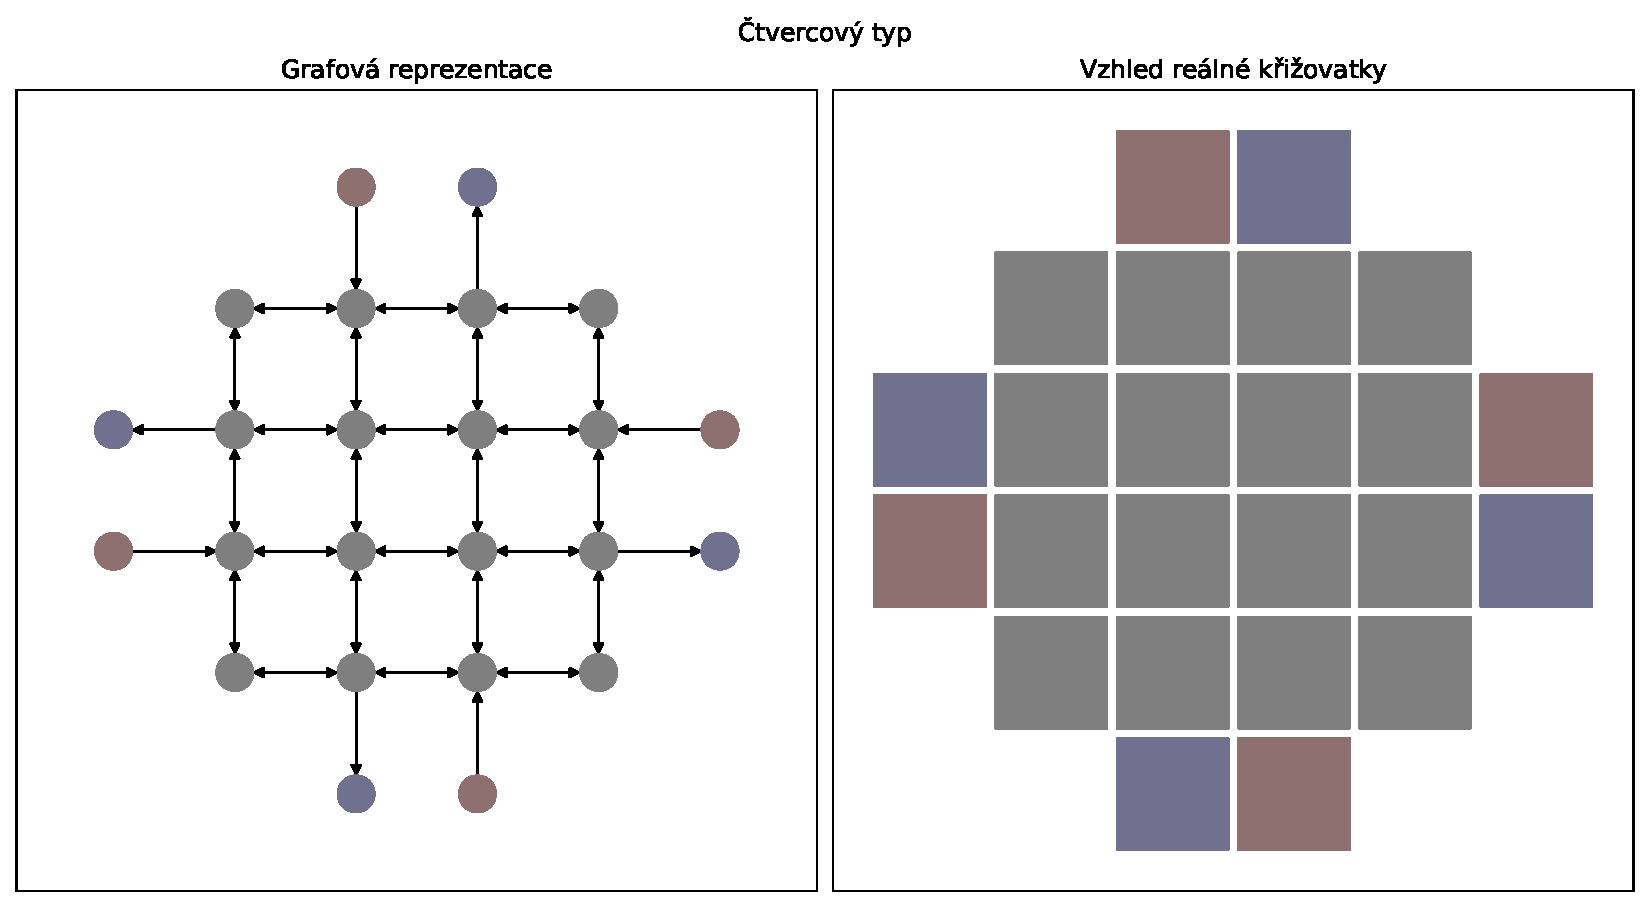
\includegraphics[width=\textwidth]{../img/Square_grid}
	\caption{Ukázka čtvercového typu křižovatky.}
	\label{fig:square_type_graph}
\end{figure}

\subsection{Oktagonální typ}\label{subsec:octagonalni-typ}

\emph{Oktagonální typ} křižovatky vychází z~\emph{typu čtvercového}, avšak rozšiřuje tento typ o~možnost diagonální jízdy.
Tohoto efektu docílí křižovatka přidáním dodatečných vrcholů mezi každé čtvercové bloky dotýkající se rohem.
Z~vizuálního hlediska se ze~čtvercových bloků stanou oktagonální (osmiúhelníkové), odtud plyne samostatný název tohoto typu.
Tyto bloky mohou mít až~$8$~sousedů.
Mezi těmito oktagonálními bloky vzniknou nové bloky reprezentující diagonální přejezdy.
Nově vytvořené bloky mají nanejvýše $4$~sousedy, tvoří tudíž pomyslný čtverec otočený o~$45^{\circ}$.
Z~významového hlediska byly odstraněny rohové bloky.

Vjezdy a výjezdy jsou totožné jako u~\emph{čtvercového typu}.

\emph{Granularita}, \emph{vjezdy} a \emph{výjezdy} mají stejný význam jako u čtvercového typu.
Počet vrcholů u~této křižovatky činí $g^2 - 4 + (g-1)^2 + 4i + 4o = 2g^2 - 2g - 3 + 4(i + o)$,
kde $g$ je granularita, $i$ počet \emph{vjezdů} a $o$ počet výjezdů.
\emph{Velikost bloku} je vzdálenost mezi dvěma sousedními vrcholy reprezentujícími oktagonální blok.
Tudíž totožná s~\emph{velikostí bloku} u~\emph{čtvercového typu}.

Doba přejezdu mezi dvěma bloky je konstantní a trvá jeden krok, ačkoliv ujeté vzdálenosti mezi vrcholy se mohou lišit.

Na~obrázku (Obrázek~\ref{fig:octagonal_type_graph}) je znázorněn příklad oktogonálního typu křižovatky s~\emph{granularitou}~$4$,
jedním \emph{vjezdem} a jedním \emph{výjezdem}.

Barvy vrcholů a bloků jsou stejné jako u~čtvercového typu, šedou barvou jsou označeny vrcholy značící běžnou plochu křižovatky,
červeno-šedou barvou označeny vrcholy reprezentující vjezdy a modro-šedé vrcholy reprezentují výjezdy.

\begin{figure}[h]
	\centering
	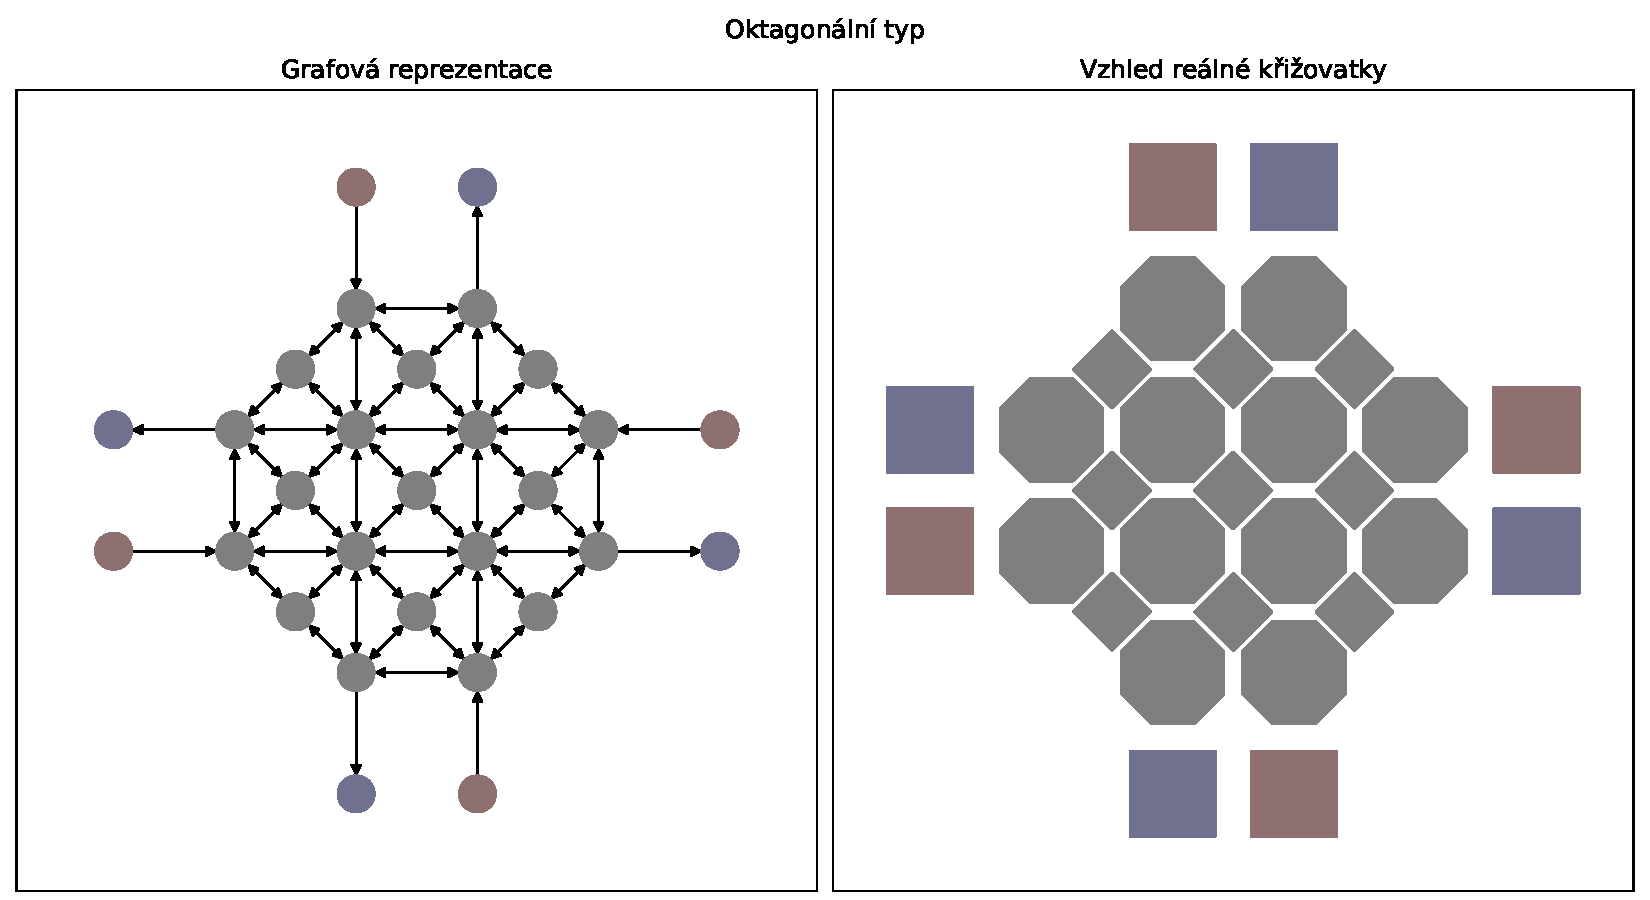
\includegraphics[width=\textwidth]{../img/Octagonal_grid}
	\caption{Ukázka oktagonálního typu křižovatky.}
	\label{fig:octagonal_type_graph}
\end{figure}

\subsection{Hexagonální typ}\label{subsec:hexagonalni-typ}

\emph{Hexagonální typ} je tvořen bloky s~tvary hexagonu (šestiúhelníku).
Každý blok má tedy až~$6$~sousedů.
Tyto bloky tvoří dohromady plochu tvaru velkého hexagonu.
Díky této reprezentaci má křižovatka tohoto typu $6$~\emph{směrů} odkud mohou auta přijíždět.

Toto rozdělení sebou nese jednu velkou nevýhodu.
Pokud chce auto jet rovně skrze křižovatku (do~protilehlého směru), křižovatka mu nemůže nabídnout rovnou cestu.

\emph{Granularita} u~tohoto typu značí počet bloků na~jedné straně \emph{plochy}.
Hodnota je taktéž rovna počtu vrcholů z~kraje křižovatky do~středu.
Počet vrcholů grafu tedy činí $6 \times g \times (g-1) + 6i + 6o$,
kde $g$ je \emph{granularita}, $i$ počet \emph{vjezdů} a $o$ počet \emph{výjezdů}.
\emph{Velikost bloku} je vzdálenost mezi dvěma sousedními vrcholy.

Na~obrázku (Obrázek~\ref{fig:hexagonal_type_graph}) je znázorněn příklad oktogonálního typu křižovatky s~\emph{granularitou}~$4$,
jedním \emph{vjezdem} a jedním \emph{výjezdem}.

Barvy vrcholů a bloků jsou opět stejné.
Šedou barvou jsou označeny vrcholy značící běžnou plochu křižovatky,
červeno-šedou barvou označeny vrcholy reprezentující vjezdy a modro-šedé vrcholy reprezentují výjezdy.

\begin{figure}[h]
	\centering
	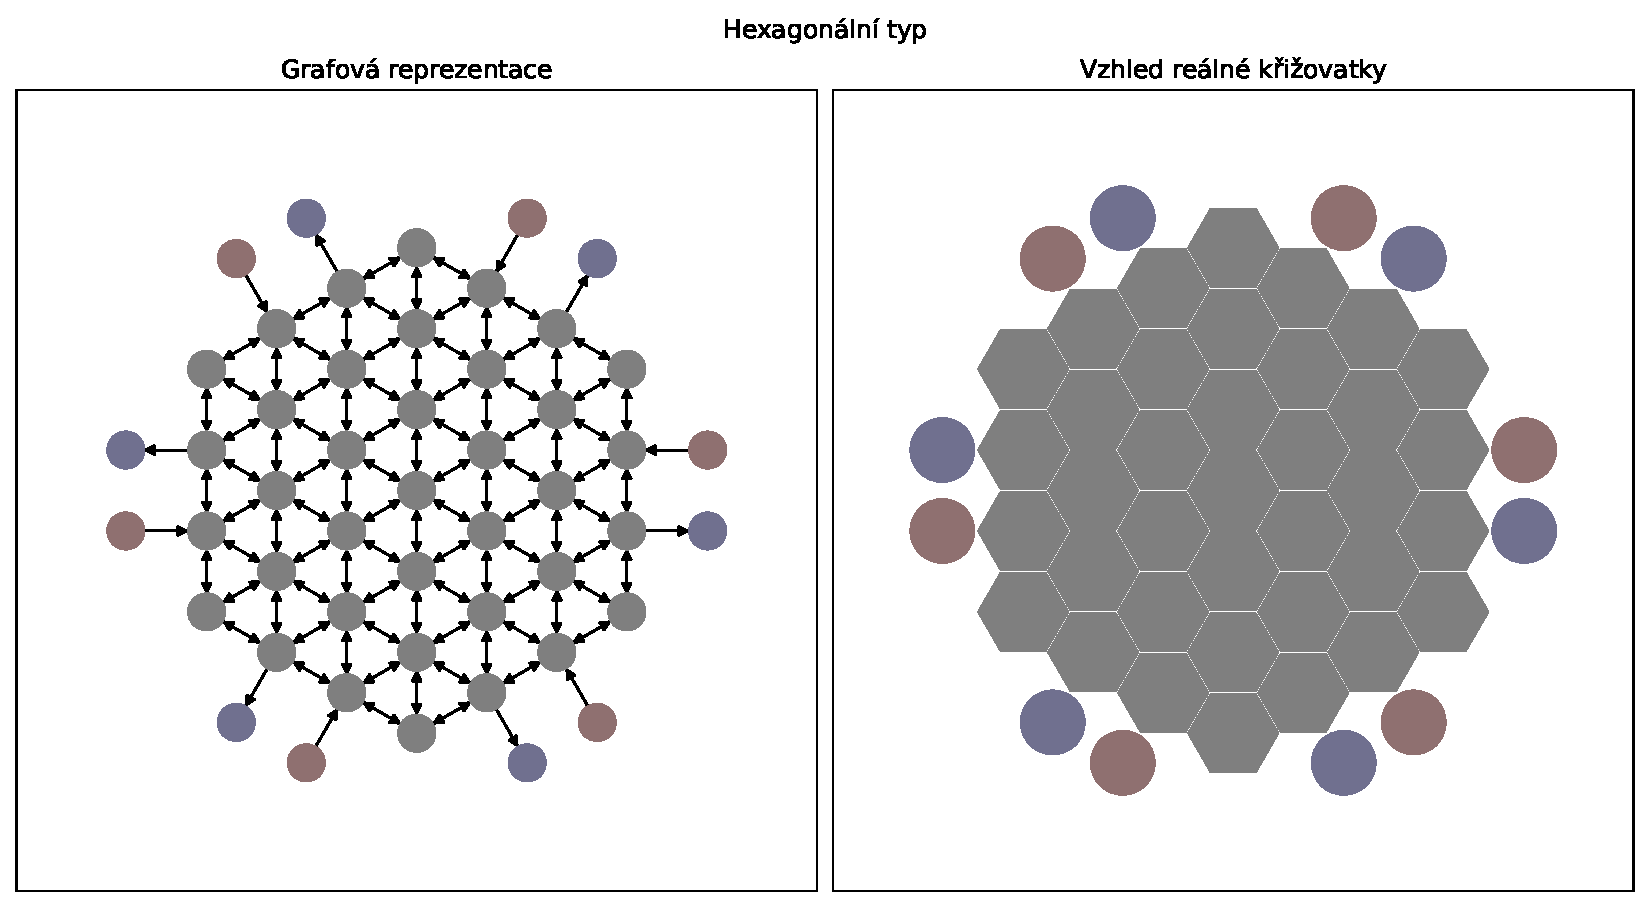
\includegraphics[width=\textwidth]{../img/Hexagonal_grid}
	\caption{Ukázka hexagonálního typu křižovatky.}
	\label{fig:hexagonal_type_graph}
\end{figure}
